\documentclass[mstat,12pt]{unswthesis}


\newlength{\cslhangindent}
\setlength{\cslhangindent}{1.5em}
\newenvironment{CSLReferences}%
  {}%
  {\par}

\usepackage{pgfgantt}
\def\tightlist{}

%%%%%%%%%%%%%%%%%%%%%%%%%%%%%%%%%%%%%%%%%%%%%%%%%%%%%%%%%%%%%%%%%%
% 
% OK...Now we get to some actual input.  The first part sets up
% the title etc that will appear on the front page
%
%%%%%%%%%%%%%%%%%%%%%%%%%%%%%%%%%%%%%%%%%%%%%%%%%%%%%%%%%%%%%%%%%

\title{Group Project Plan by Group K\\[0.5cm]Impact of Climate Change on
Electricity Consumption in New South Wales}

\authornameonly{Abdelrhman Dameen (z5427841), Md Nezam Uddin
(z5339862), Pam Moodley (z5366156), Van Hai Ho (z3071030) }

\author{\Authornameonly}

\copyrightfalse
\figurespagefalse
\tablespagefalse

%%%%%%%%%%%%%%%%%%%%%%%%%%%%%%%%%%%%%%%%%%%%%%%%%%%%%%%%%%%%%%%%%
%
%  And now the document begins
%  The \beforepreface and \afterpreface commands puts the
%  contents page etc in
%
%%%%%%%%%%%%%%%%%%%%%%%%%%%%%%%%%%%%%%%%%%%%%%%%%%%%%%%%%%%%%%%%%%


%%%%%%%%%%%%%%%%%%%%%%%%%%%%%%%%%%%%%%%%%%%%%%%%%%%%%%%%%%%%%%%%%%%%%%%
%
%  A small sample UNSW Coursework Masters thesis file.
%  Any questions to Ian Doust i.doust@unsw.edu.au and/or Gery Geenens ggeenens@unsw.edu.au
%
%%%%%%%%%%%%%%%%%%%%%%%%%%%%%%%%%%%%%%%%%%%%%%%%%%%%%%%%%%%%%%%%%%%%%%%
%
%  The first part pulls in a UNSW Thesis class file.  This one is
%  slightly nonstandard and has been set up to do a couple of
%  things automatically
%
 
%%%%%%%%%%%%%%%%%
%% Precisely one of the next four lines should be uncommented.
%% Choose the one which matches your degree, uncomment it, and comment out the other two!
%\documentclass[mfin,12pt]{unswthesis}    %%  For Master of Financial Mathematics 
%\documentclass[mmath,12pt]{unswthesis}   %%  For Master of Mathematics
%\documentclass[mstat,12pt]{unswthesis}  %%  For Master of Statistics
%%%%%%%%%%%%%%%%%



\linespread{1}
\usepackage{amsfonts}
\usepackage{amssymb}
\usepackage{amsthm}
\usepackage{latexsym,amsmath}
\usepackage{graphicx}
\usepackage{afterpage}
\usepackage[colorlinks]{hyperref}
 \hypersetup{
     colorlinks=true,
     linkcolor=blue,
     filecolor=blue,
     citecolor= black,      
     urlcolor=cyan,
     }
\usepackage{textcomp}
\usepackage{longtable}
\usepackage{booktabs}
\usepackage{float}

%%%%%%%%%%%%%%%%%%%%%%%%%%%%%%%%%%%%%%%%%%%%%%%%%%%%%%%%%%%%%%%%%
%
%  The following are some simple LaTeX macros to give some
%  commonly used letters in funny fonts. You may need more or less of
%  these
%
\newcommand{\R}{\mathbb{R}}
\newcommand{\Q}{\mathbb{Q}}
\newcommand{\C}{\mathbb{C}}
\newcommand{\N}{\mathbb{N}}
\newcommand{\F}{\mathbb{F}}
\newcommand{\PP}{\mathbb{P}}
\newcommand{\T}{\mathbb{T}}
\newcommand{\Z}{\mathbb{Z}}
\newcommand{\B}{\mathfrak{B}}
\newcommand{\BB}{\mathcal{B}}
\newcommand{\M}{\mathfrak{M}}
\newcommand{\X}{\mathfrak{X}}
\newcommand{\Y}{\mathfrak{Y}}
\newcommand{\CC}{\mathcal{C}}
\newcommand{\E}{\mathbb{E}}
\newcommand{\cP}{\mathcal{P}}
\newcommand{\cS}{\mathcal{S}}
\newcommand{\A}{\mathcal{A}}
\newcommand{\ZZ}{\mathcal{Z}}
%%%%%%%%%%%%%%%%%%%%%%%%%%%%%%%%%%%%%%%%%%%%%%%%%%%%%%%%%%%%%%%%%%%%%
%
% The following are much more esoteric commands that I have left in
% so that this file still processes. Use or delete as you see fit
%
\newcommand{\bv}[1]{\mbox{BV($#1$)}}
\newcommand{\comb}[2]{\left(\!\!\!\begin{array}{c}#1\\#2\end{array}\!\!\!\right)
}
\newcommand{\Lat}{{\rm Lat}}
\newcommand{\var}{\mathop{\rm var}}
\newcommand{\Pt}{{\mathcal P}}
\def\tr(#1){{\rm trace}(#1)}
\def\Exp(#1){{\mathbb E}(#1)}
\def\Exps(#1){{\mathbb E}\sparen(#1)}
\newcommand{\floor}[1]{\left\lfloor #1 \right\rfloor}
\newcommand{\ceil}[1]{\left\lceil #1 \right\rceil}
\newcommand{\hatt}[1]{\widehat #1}
\newcommand{\modeq}[3]{#1 \equiv #2 \,(\text{mod}\, #3)}
\newcommand{\rmod}{\,\mathrm{mod}\,}
\newcommand{\p}{\hphantom{+}}
\newcommand{\vect}[1]{\mbox{\boldmath $ #1 $}}
\newcommand{\reff}[2]{\ref{#1}.\ref{#2}}
\newcommand{\psum}[2]{\sum_{#1}^{#2}\!\!\!'\,\,}
\newcommand{\bin}[2]{\left( \begin{array}{@{}c@{}}
				#1 \\ #2
			\end{array}\right)	}
%
%  Macros - some of these are in plain TeX (gasp!)
%
\newcommand{\be}{($\beta$)}
\newcommand{\eqp}{\mathrel{{=}_p}}
\newcommand{\ltp}{\mathrel{{\prec}_p}}
\newcommand{\lep}{\mathrel{{\preceq}_p}}
\def\brack#1{\left \{ #1 \right \}}
\def\bul{$\bullet$\ }
\def\cl{{\rm cl}}
\let\del=\partial
\def\enditem{\par\smallskip\noindent}
\def\implies{\Rightarrow}
\def\inpr#1,#2{\t \hbox{\langle #1 , #2 \rangle} \t}
\def\ip<#1,#2>{\langle #1,#2 \rangle}
\def\lp{\ell^p}
\def\maxb#1{\max \brack{#1}}
\def\minb#1{\min \brack{#1}}
\def\mod#1{\left \vert #1 \right \vert}
\def\norm#1{\left \Vert #1 \right \Vert}
\def\paren(#1){\left( #1 \right)}
\def\qed{\hfill \hbox{$\Box$} \smallskip}
\def\sbrack#1{\Bigl \{ #1 \Bigr \} }
\def\ssbrack#1{ \{ #1 \} }
\def\smod#1{\Bigl \vert #1 \Bigr \vert}
\def\smmod#1{\bigl \vert #1 \bigr \vert}
\def\ssmod#1{\vert #1 \vert}
\def\sspmod#1{\vert\, #1 \, \vert}
\def\snorm#1{\Bigl \Vert #1 \Bigr \Vert}
\def\ssnorm#1{\Vert #1 \Vert}
\def\sparen(#1){\Bigl ( #1 \Bigr )}

\newcommand\blankpage{%
    \null
    \thispagestyle{empty}%
    \addtocounter{page}{-1}%
    \newpage}

%%%%%%%%%%%%%%%%%%%%%%%%%%%%%%%
%
% These environments allow you to get nice numbered headings
%  for your Theorems, Definitions etc.  
%
%  Environments
%
%%%%%%%%%%%%%%%%%%%%%%%%%%%%%%%

\newtheorem{theorem}{Theorem}[section]
\newtheorem{lemma}[theorem]{Lemma}
\newtheorem{proposition}[theorem]{Proposition}
\newtheorem{corollary}[theorem]{Corollary}
\newtheorem{conjecture}[theorem]{Conjecture}
\newtheorem{definition}[theorem]{Definition}
\newtheorem{example}[theorem]{Example}
\newtheorem{remark}[theorem]{Remark}
\newtheorem{question}[theorem]{Question}
\newtheorem{notation}[theorem]{Notation}
\numberwithin{equation}{section}

%%%%%%%%%%%%%%%%%%%%%%%%%%%%%%%%%%%%%%%%%%%%%%%%%%%%%%%%%%%%%%%%%%
%
%  If you've got some funny special words that LaTeX might not
% hyphenate properly, you can give it a helping hand:
%

\hyphenation{Mar-cin-kie-wicz Rade-macher}


\newlength{\cslhangindent}
\setlength{\cslhangindent}{1.5em}
\newlength{\csllabelwidth}
\setlength{\csllabelwidth}{3em}
\newenvironment{CSLReferences}[2] % #1 hanging-ident, #2 entry spacing
 {% don't indent paragraphs
  \setlength{\parindent}{0pt}
  % turn on hanging indent if param 1 is 1
  \ifodd #1 \everypar{\setlength{\hangindent}{\cslhangindent}}\ignorespaces\fi
  % set entry spacing
  \ifnum #2 > 0
  \setlength{\parskip}{#2\baselineskip}
  \fi
 }%
 {}
\usepackage{calc} % for \widthof, \maxof
\newcommand{\CSLBlock}[1]{#1\hfill\break}
\newcommand{\CSLLeftMargin}[1]{\parbox[t]{\maxof{\widthof{#1}}{\csllabelwidth}}{#1}}
\newcommand{\CSLRightInline}[1]{\parbox[t]{\linewidth}{#1}}
\newcommand{\CSLIndent}[1]{\hspace{\cslhangindent}#1}

\bibliographystyle{elsarticle-num}




\begin{document}

\beforepreface

\prefacesection{Abstract}

Climate Change has had significant impacts on our everyday life around
the world. Energy consumption is essential in modern life, required by
individual family units to large organizations and industrial scales. In
this project, we investigate a strategy for integrative demand
forecasting for energy consumption using a machine learning approach
with seasonal decomposition and climate change impact analysis.

%\afterpage{\blankpage}


\afterpreface





%%%%%%%%%%%%%%%%%%%%%%%%%%%%%%%%%%%%%%%%%%%%%%%%%%%%%%%%%%%%%%%%%%
%
% Now we can start on the first chapter
% Within chapters we have sections, subsections and so forth
%
%%%%%%%%%%%%%%%%%%%%%%%%%%%%%%%%%%%%%%%%%%%%%%%%%%%%%%%%%%%%%%%%%%



%%%%%%%%%%%%%%%%%%%%%%%%%%%%%%%%%%%%%

%\afterpage{\blankpage}


\setcounter{chapter}{1}
\renewcommand\thesection{\arabic{section}}

\hypertarget{introduction-and-motivation}{%
\section{Introduction and
Motivation}\label{introduction-and-motivation}}

The supply and demand of energy are volatile. For suppliers to enter and
remain in the market, the supply of energy must be profitable.
Profitability hinges on accurately predicting and providing the most
efficient amount of energy to the grid.

It is a known fact that weather plays a significant role in energy
demand. For instance, heating is utilized when the temperature drops,
and air conditioning is used when the temperature rises. Therefore, this
analysis will examine the impact of weather on energy demand to better
predict the required supply. If the supply is not accurately calculated,
suppliers may incur excessive costs to provide additional energy. Given
the substantial role of weather in energy demand, the analysis will also
consider the effects of global warming and erratic storm periods.

Other factors also influence the supply and demand of energy. This
project will attempt to identify the patterns that daily and seasonal
variations, as well as holidays, have on demand.

Incorporating all these factors into an analysis of energy demand will
highlight the advantages of using a machine learning model to predict
demand more efficiently.

Specifically, within the scope of this project, we will identify energy
consumption patterns to uncover hidden temporal trends in demand,
including daily and seasonal fluctuations. We will perform a climate
impact assessment to quantify how changes in climate variables, like
temperature, affect energy demand.

Additionally, we will conduct holiday and special event analysis to
understand their impact on energy consumption, thereby aiding in better
planning.

Based on this analysis, we will provide policy recommendations to offer
actionable insights for energy policy formulation, including the
diversification of energy sources to balance demand. We will create a
machine learning model capable of predicting future energy demand with
high accuracy, incorporating all the identified variables.

\hypertarget{brief-literature-review}{%
\section{Brief Literature Review}\label{brief-literature-review}}

The topic of how climate change impacts residential energy use has been
studied in various global contexts. The first research paper
investigates the potential changes in energy consumption in Europe and
Australia, predicting a variable impact ranging from a 26\% decrease to
a whopping 350\% increase by the year 2100. {[}1{]}. Particularly, homes
in Sydney have been identified as more susceptible to climate change,
emphasizing the importance of geographical factors. Another study shifts
the focus to Asia, particularly to five major cities in China. This
research expects an increase in cooling energy demands while foreseeing
a decrease in heating requirements {[}2{]}. These trends align with the
general narrative that global warming is driving cooling needs upwards.
Finally, a third study zeroes in on Brazil, forecasting an upsurge in
energy demands by up to 185\% by 2080. However, the paper also proposes
that passive design techniques could significantly mitigate these energy
demands, potentially reducing annual consumption by up to 50\% {[}3{]}.

Collectively, these studies underline that climate change will have a
substantial impact on residential and office energy demands worldwide.
They stress the significance of local geographical and climatic
conditions and propose passive design as a key strategy for mitigating
future energy needs.

\hypertarget{methods-software-and-data-description}{%
\section{Methods, Software and Data
Description}\label{methods-software-and-data-description}}

Regression analysis will be utilized to determine the relationship
between the attributes of temperature, global warming, holidays, and
days of the week against demand.

Python and R/Rsudio software will be used to analyse the data. Libraries
and packages such as pandas, matplotlib, seaborn for Python and ggplot2,
dplyr, caret for R are required in this analysis. RMarkdown, knitr will
also be utilized for putting the analysis together.

The data provided contains energy demand data in 5-minute intervals from
January 1, 2010, to August 1, 2022, for New South Wales. The data is in
a comma-delimited file format, with columns labeled Datetime, RegionId,
and TotalDemand. The RegionId consists only of NSW1.

The temperature data is in 30-minute intervals from January 1, 2010, to
August 1, 2022, for New South Wales. The data is provided in a
comma-delimited file format, with headings DateTime, Location, and
Temperature (in Celsius). The source of the temperature data is the
Bankstown weather location. Invalid temperatures, such as -9999, will be
removed from the analysis.

The data will need further analysis and cleaning, including the removal
of invalid and outlier data.

When merging these datasets, there will be mismatched data since the
demand is in 5-minute intervals and the temperature data is in 30-minute
intervals. There are approximately 1.3 million rows of demand data and
247,646 rows of temperature data; therefore, some analysis is required
to map more demand data to temperature data. One possibility is to
simulate temperature data for the data points that are not available.

Since this project aims to address questions regarding future energy
demand, historical data will be utilized, and the datasets provided are
an excellent starting point. Additional data will be sourced to enhance
these datasets.

\hypertarget{activities-and-schedule}{%
\section{Activities and Schedule}\label{activities-and-schedule}}

\hypertarget{main-tasks-and-activities}{%
\subsection{Main tasks and activities}\label{main-tasks-and-activities}}

To achieve the objectives discussed in the previous sections, the
following main tasks and activities will need to be completed:

\begin{itemize}
\tightlist
\item
  Project planning.
\item
  Performing literature reviews.
\item
  Assessing the provided data set, including: temperature\_nsw.csv and
  totaldemand\_nsw.csv.
\item
  Researching algorithms: Identifying appropriate machine learning
  algorithms to use for the project.
\item
  Data cleaning: Identifying and excluding irrelevant data from the
  provided data set.
\item
  Data enriching: Identifying additional data to integrate with and
  enrich the provided data set.
\item
  Data integration: Combining and integrating the provided data sets
  with additional data.
\item
  Performing data analysis using machine learning algorithms.
\item
  Analyzing the output and providing recommendations.
\item
  Creating visualizations to communicate the findings from the analysis.
\item
  Writing the report.
\item
  Creating video presentations.
\end{itemize}

\hypertarget{activities-and-schedule-1}{%
\subsection{Activities and Schedule}\label{activities-and-schedule-1}}

The skill sets within our group are diverse. Each team member possesses
skills that complement one another, as illustrated in the Mind Map
located in the Appendix section. Based on these skill sets, we have
allocated tasks accordingly.

We plan to perform data cleaning, enrichment, and integration during
Weeks 2 and 3. Data mining to uncover patterns and hidden relationships
in the datasets will take place in Weeks 3 and 4.

Following these discoveries, a new plan will be implemented based on the
data and analyses found. Decisions regarding useful visualizations will
be noted as the project progresses. We will also gather more research
and acquire an in-depth understanding to enrich our analysis.

Our aim is to complete all analyses and draw conclusions by the end of
Week 4. Weeks 5 and 6 will be dedicated to refining the report and
creating video presentations.

Below is a detailed timetable for the main project activities. The team
member listed first for each activity is the primary owner and is
responsible for completing that particular task:

\begin{table}[!ht]
\begin{center}
\begin{tabular}{|l|c|c|c|}
\hline
Activity & Owner & Start Date & EndDate \\
\hline
Project Planning & All & Week 1 & Week 2 \\
\hline
Perform literature reviews & All & Week 2 & Week 2 \\
\hline
Assess the provided data set & All & Week 2 & Week 2 \\
\hline
Research algorithms & Abdo + Nezam & Week 2 & Week 3 \\
\hline
Data cleaning & Van + Pam & Week 2 & Week 3 \\
\hline
Data enriching & Pam + Van & Week 2 & Week 3 \\
\hline
Data integration & Van + Pam & Week 2 & Week 3 \\
\hline
Perform data analysis & Abdo + Nezam & Week 3 & Week 4 \\
\hline
Analyse the output & Nezam + Abdo & Week 3 & Week 4 \\
\hline
Create visualisations & Pam + Abdo & Week 3 & Week 4 \\
\hline
Write report & All & Week 5 & Week 6 \\
\hline
Create video presentations & All & Week 5 & Week 6 \\
\hline
\end{tabular}
\caption{\label{activity-schedule-table}Activity and Schedule}
\end{center}
\end{table}

More details on our activities and schedule are presented in the Gantt
Chart in the Appendix section.

\hypertarget{appendix}{%
\chapter*{Appendix}\label{appendix}}
\addcontentsline{toc}{chapter}{Appendix}

Below are the skill sets that each team member possesses. Based on
these, we have distributed the work accordingly.

\begin{figure}[ht]
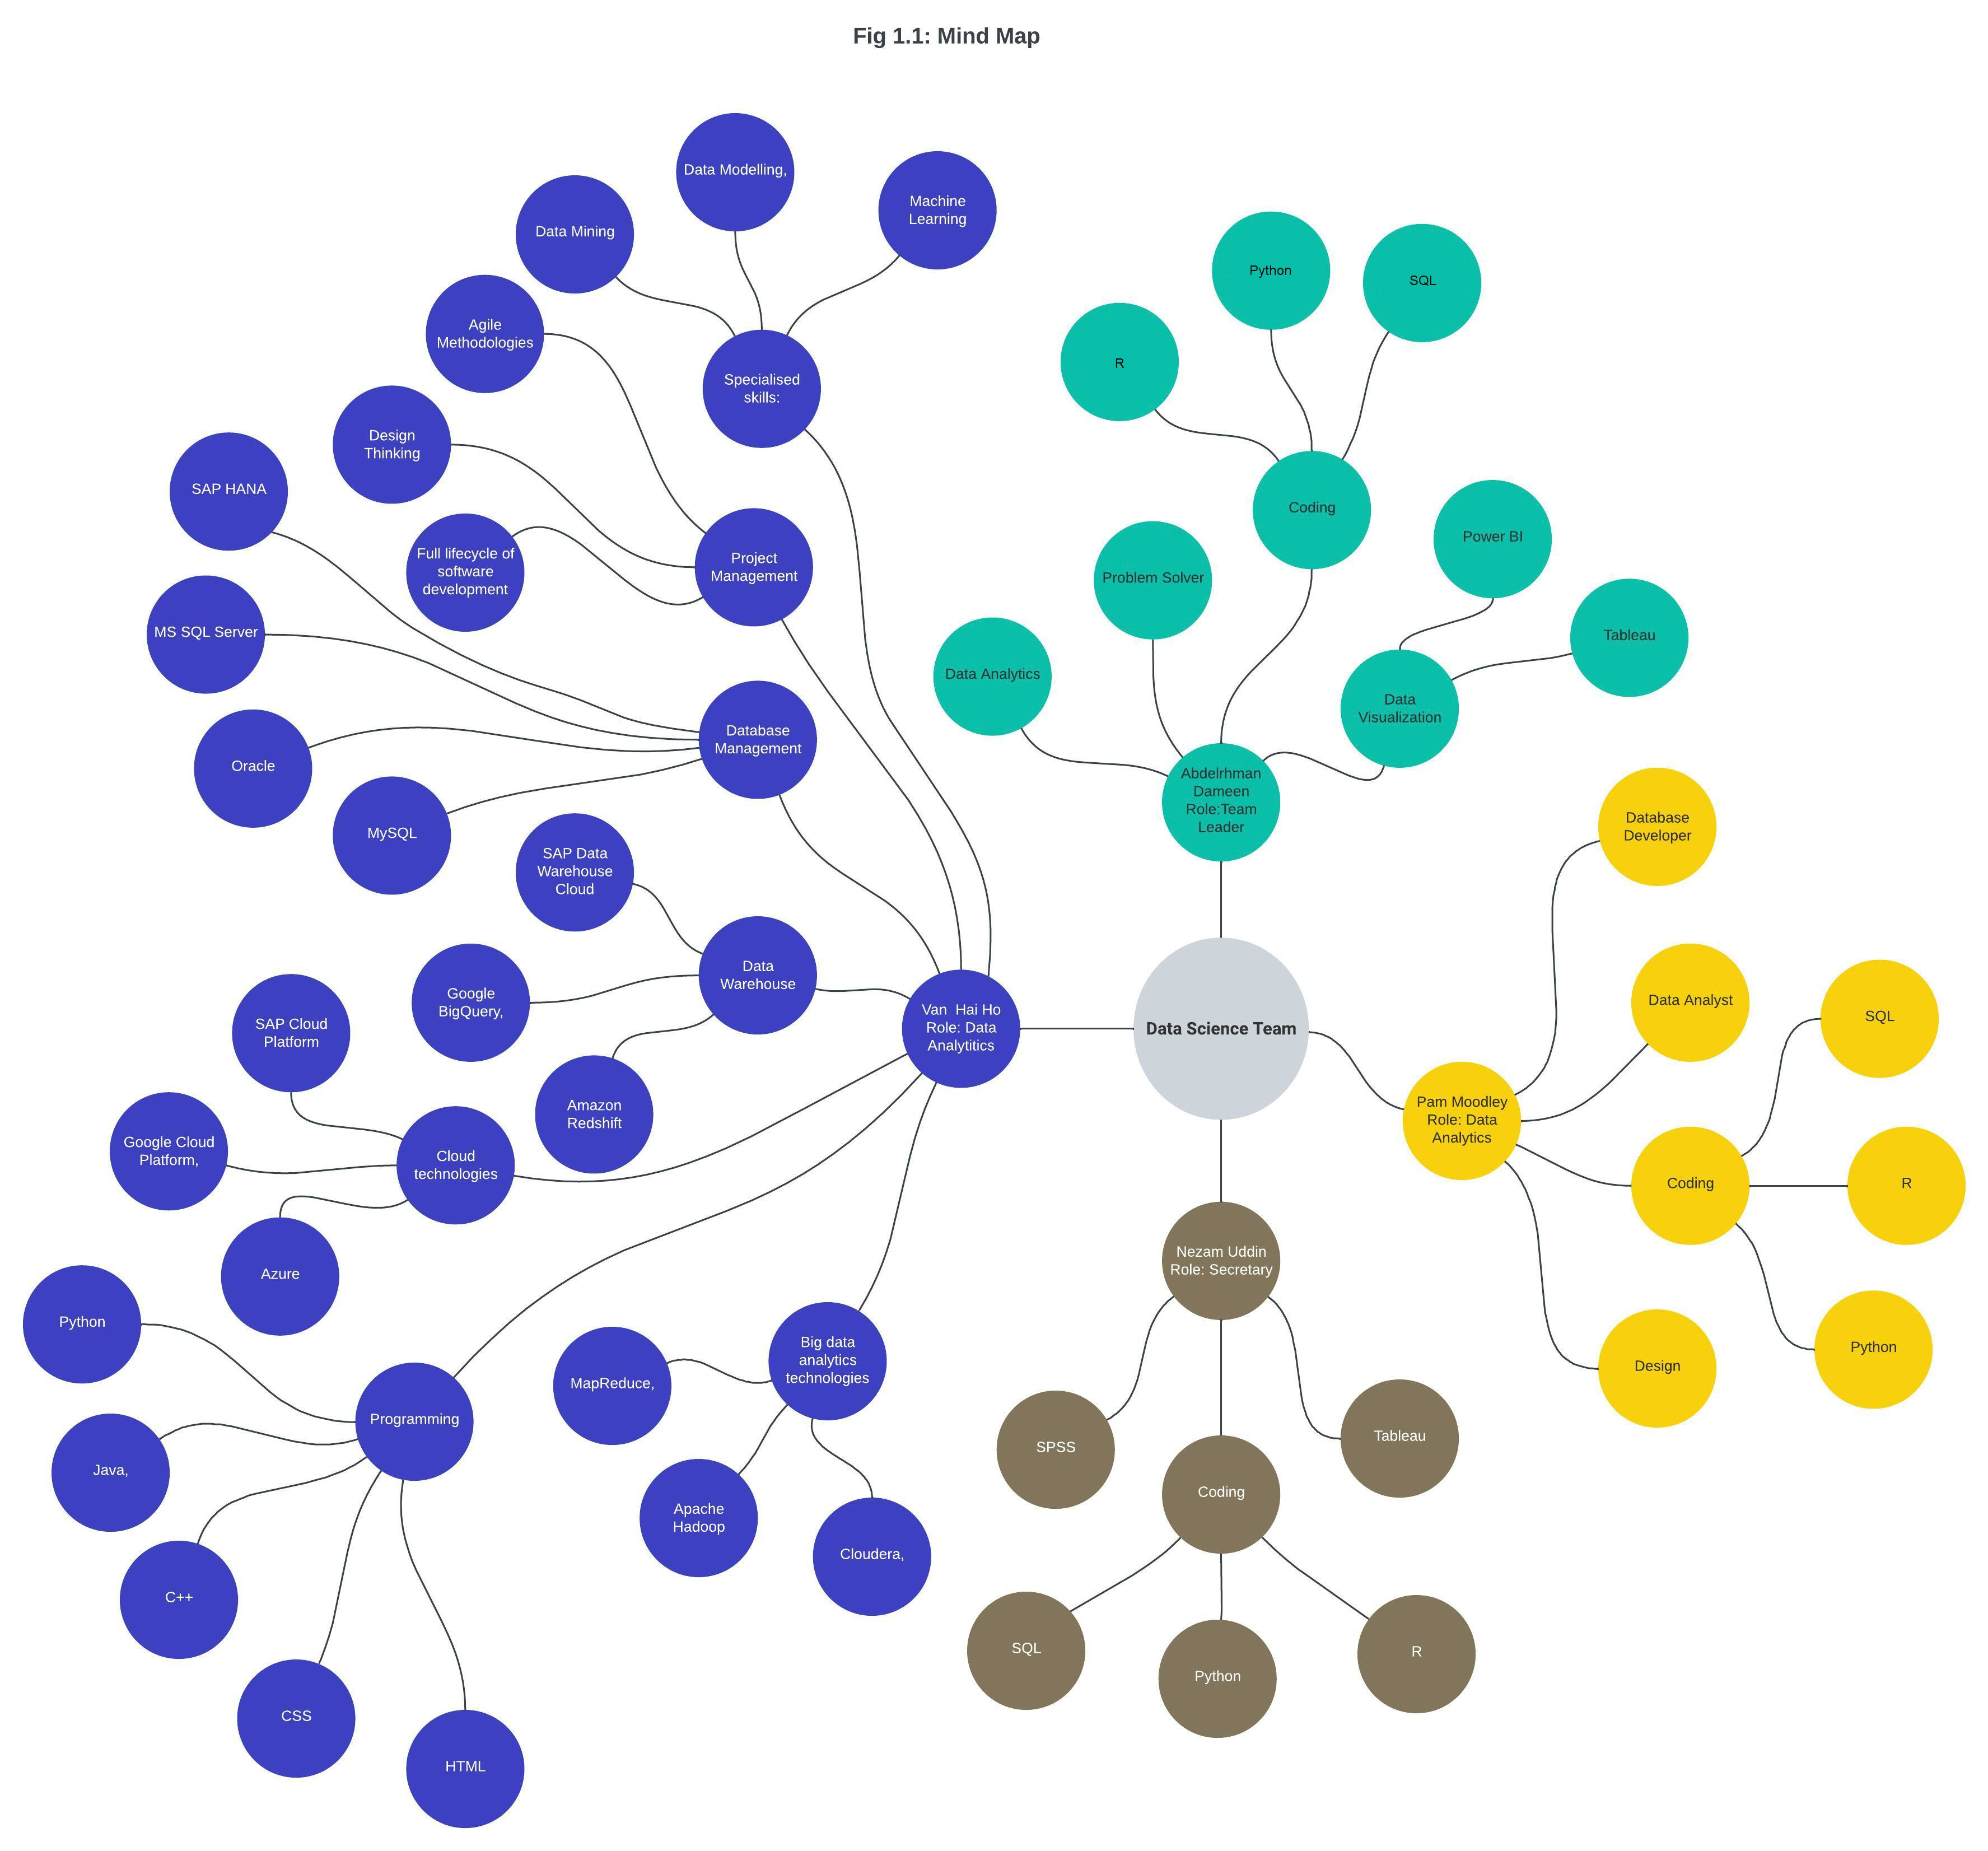
\includegraphics[width = \textwidth, height=!]{images/ZZSC9020_Group_K_skillsets.jpeg}
\centering
\caption{ZZSC9020 Group K skill sets}
\end{figure}

Our activities and schedule are represented in the following Gantt
Chart:

\definecolor{barblue}{RGB}{153,204,254}
\definecolor{groupblue}{RGB}{51,102,254}
\definecolor{linkred}{RGB}{165,0,33}
\renewcommand\sfdefault{phv}
\renewcommand\mddefault{mc}
\renewcommand\bfdefault{bc}
\setganttlinklabel{s-s}{START-TO-START}
\setganttlinklabel{f-s}{FINISH-TO-START}
\setganttlinklabel{f-f}{FINISH-TO-FINISH}
\sffamily
\begin{ganttchart}[
    canvas/.append style={fill=none, draw=black!5, line width=.75pt},
    hgrid style/.style={draw=black!5, line width=.75pt},
    vgrid={*1{draw=black!5, line width=.75pt}},
    today=1,
    today rule/.style={
      draw=black!64,
      dash pattern=on 3.5pt off 4.5pt,
      line width=1.5pt
    },
    today label font=\small\bfseries,
    title/.style={draw=none, fill=none},
    title label font=\bfseries\footnotesize,
    title label node/.append style={below=7pt},
    include title in canvas=false,
    bar label font=\mdseries\small\color{black!70},
    bar label node/.append style={left=0.5cm},
    bar/.append style={draw=none, fill=black!63},
    bar incomplete/.append style={fill=barblue},
    bar progress label font=\mdseries\footnotesize\color{black!70},
    group incomplete/.append style={fill=groupblue},
    group left shift=0,
    group right shift=0,
    group height=.5,
    group peaks tip position=0,
    group label node/.append style={left=.1cm},
    group progress label font=\bfseries\small,
    link/.style={-latex, line width=1.5pt, linkred},
    link label font=\scriptsize\bfseries,
    link label node/.append style={below left=-2pt and 0pt}
  ]{1}{6}
  \gantttitle[
    title label node/.append style={below left=7pt and -3pt}
  ]{WEEKS:\quad1}{1}
  \gantttitlelist{2,...,6}{1} \\
  
  \ganttgroup[progress=75]{WBS 1 Project Plan}{1}{2} \\
  \ganttbar[
    progress=75,
    name=WBS1A
  ]{\textbf{WBS 1.1} Project Plan}{1}{2} \\

  \ganttgroup[progress=10]{WBS 2 Literature Review}{2}{2} \\
  \ganttbar[progress=10]{\textbf{WBS 2.1} Literature Review}{2}{2} \\

  \ganttgroup[progress=0]{WBS 3 Data Preparation}{2}{3} \\
  \ganttbar[progress=0, name = WBS31]{\textbf{WBS 3.1} Assess provided data set}{2}{2} \\
  \ganttbar[progress=0, name = WBS32]{\textbf{WBS 3.2} Data cleaning}{2}{2} \\
  \ganttbar[progress=0, name = WBS33]{\textbf{WBS 3.3} Data enriching}{2}{3} \\
  \ganttbar[progress=0, name = WBS34]{\textbf{WBS 3.3} Data integration}{2}{3} \\

  \ganttgroup[progress=0]{WBS 4 Data Analysis}{3}{4} \\
  \ganttbar[progress=0, name = WBS41]{\textbf{WBS 4.1} Apply algorithms}{3}{4} \\
  \ganttbar[progress=0, name = WBS42]{\textbf{WBS 4.2} Analyse output}{3}{4} \\

  \ganttgroup[progress=0]{WBS 5 Report and Presentation}{5}{6} \\
  \ganttbar[progress=0, name = WBS51]{\textbf{WBS 5.1} Create visualisation}{5}{6} \\
  \ganttbar[progress=0, name = WBS52]{\textbf{WBS 5.2} Write report}{5}{6} \\
  \ganttbar[progress=0, name = WBS53]{\textbf{WBS 5.3} Create video presentation}{5}{6} \\
  
  \ganttlink[link type=s-s]{WBS31}{WBS32}
  \ganttlink[link type=f-f]{WBS33}{WBS34}
  \ganttlink[link type=s-s]{WBS34}{WBS41}
  \ganttlink[link type=s-s]{WBS41}{WBS42}
  \ganttlink[link type=f-s]{WBS42}{WBS51}
  \ganttlink[link type=f-s]{WBS42}{WBS52}
  \ganttlink[link type=f-s]{WBS42}{WBS53}

\end{ganttchart}

\hypertarget{references}{%
\chapter*{References}\label{references}}
\addcontentsline{toc}{chapter}{References}

\bibliographystyle{elsarticle-num}
\bibliography{references}

\hypertarget{refs}{}
\begin{CSLReferences}{0}{0}
\leavevmode\vadjust pre{\hypertarget{ref-Yazdan-et-al-2022-FC}{}}%
1. Yazdan MMS, Khosravia M, Saki S, Mehedi MAA. Forecasting energy
consumption time series using recurrent neural network in tensorflow.
2022.

\leavevmode\vadjust pre{\hypertarget{ref-Fard-Hosseini-2022-ML}{}}%
2. Fard RH, Hosseini S. Machine learning algorithms for prediction of
energy consumption and IoT modeling in complex networks. Microprocessors
and Microsystems. 2022;89.

\leavevmode\vadjust pre{\hypertarget{ref-Invidiata-Ghisi-2016-CC}{}}%
3. Invidiata A, Ghisi E. Impact of climate change on heating and cooling
energy demand in houses in brazil. Energy and Buildings.
2016;130:20--32.

\end{CSLReferences}







\end{document}

